%%
%% This is file `sample-sigconf.tex',
%% generated with the docstrip utility.
%%
%% The original source files were:
%%
%% samples.dtx  (with options: `sigconf')
%% 
%% IMPORTANT NOTICE:
%% 
%% For the copyright see the source file.
%% 
%% Any modified versions of this file must be renamed
%% with new filenames distinct from sample-sigconf.tex.
%% 
%% For distribution of the original source see the terms
%% for copying and modification in the file samples.dtx.
%% 
%% This generated file may be distributed as long as the
%% original source files, as listed above, are part of the
%% same distribution. (The sources need not necessarily be
%% in the same archive or directory.)
%%
%%
%% Commands for TeXCount
%TC:macro \cite [option:text,text]
%TC:macro \citep [option:text,text]
%TC:macro \citet [option:text,text]
%TC:envir table 0 1
%TC:envir table* 0 1
%TC:envir tabular [ignore] word
%TC:envir displaymath 0 word
%TC:envir math 0 word
%TC:envir comment 0 0
%%
%%
%% The first command in your LaTeX source must be the \documentclass command.
\documentclass[sigconf]{acmart}

%%% Customisation
% Determine whether it is local compilation or overleaf compilation
\makeatletter
\begingroup\endlinechar=-1\relax
       \everyeof{\noexpand}%
       \edef\x{\endgroup\def\noexpand\homepath{%
         \@@input|"kpsewhich --var-value=HOME" }}\x
\makeatother
\def\overleafhome{/tmp}% change as appropriate

% Include algorithm.
\usepackage{cleveref}
\usepackage[ruled,linesnumbered]{algorithm2e}

% Global change of algorithm input output naming.
\SetKwInput{KwData}{Input}
\SetKwInput{KwResult}{Output}

% Color words red.
\usepackage{xcolor}
%%% End customisation


%%
%% \BibTeX command to typeset BibTeX logo in the docs
\AtBeginDocument{%
  \providecommand\BibTeX{{%
    \normalfont B\kern-0.5em{\scshape i\kern-0.25em b}\kern-0.8em\TeX}}}

%% Rights management information.  This information is sent to you
%% when you complete the rights form.  These commands have SAMPLE
%% values in them; it is your responsibility as an author to replace
%% the commands and values with those provided to you when you
%% complete the rights form.
\setcopyright{acmcopyright}
\copyrightyear{2022}
\acmYear{2022}
\acmDOI{XXXXXXX.XXXXXXX}

%% These commands are for a PROCEEDINGS abstract or paper.
\acmConference[Conference acronym 'ICONS]{International Conference on Neuromorphic Systems}{July 27--29,
  2022}{Knoxville, Tennessee}
\acmPrice{15.00}
\acmISBN{978-1-4503-XXXX-X/18/06}

% Try 1
%\newcommand\authornotemark[1][\relax]{%
%\ifx#1\relax\relax\relax
% \g@addto@macro\addresses{\@authornotemark}%
%\else
%  \g@addto@macro\addresses{\@@authornotemark{#1}}%
%\fi}
% Try 2
%\def\@authornotemark{\g@addto@macro\@currentauthors{\footnotemark\relax}}
%\@@authornotemark

% Try 3
%\def\@authornotemark{\g@addto@macro\@currentauthors{\footnotemark\relax}}
%%\@@authornotemark

% Try 4
%\def\@authornotes{}
%\def\authornote#1{%
%  \if@ACM@anonymous\else
%    \g@addto@macro\addresses{\@authornotemark}
%    \g@addto@macro\@authornotes{%
%      \stepcounter{footnote}\footnotetext{#1}}%
%  \fi}


%%
%% Submission ID.
%% Use this when submitting an article to a sponsored event. You'll
%% receive a unique submission ID from the organizers
%% of the event, and this ID should be used as the parameter to this command.
%%\acmSubmissionID{123-A56-BU3}

%%
%% The majority of ACM publications use numbered citations and
%% references.  The command \citestyle{authoryear} switches to the
%% "author year" style.
%%
%% If you are preparing content for an event
%% sponsored by ACM SIGGRAPH, you must use the "author year" style of
%% citations and references.
%% Uncommenting
%% the next command will enable that style.
%%\citestyle{acmauthoryear}

%%
%% end of the preamble, start of the body of the document source.
\begin{document}

%%
%% The "title" command has an optional parameter,
%% allowing the author to define a "short title" to be used in page headers.
\title{Leveraging brain-adaptation principles to increase radiation resistance of neuromorphic space hardware}

%%
%% The "author" command and its associated commands are used to define
%% the authors and their affiliations.
%% Of note is the shared affiliation of the first two authors, and the
%% "authornote" and "authornotemark" commands
%% used to denote shared contribution to the research.
\author{Akke Toeter}
%\authornote{All authors contributed equally to this research.}
\orcid{0000-0002-9577-920X}

\affiliation{%
  \institution{Delft University of Technology, Radboud University}
  \country{The Netherlands}
}
\email{a.h.h.toeter@tudelft.nl}

\author{J.H.P. Kwisthout}
\orcid{0000-0003-4383-7786}
%\authornotemark[1]
\affiliation{%
  \institution{Radboud University}
  \country{The Netherlands}
}
\email{j.kwisthout@donders.ru.nl}

\author{D.M. Stam}
\orcid{0000-0003-3697-2971}
\affiliation{%
  \institution{Delft University of Technology}
  \country{The Netherlands}
}
\email{D.M.Stam@tudelft.nl}

\author{A. Menicucci}
\orcid{0000-0002-7064-6275}
\affiliation{%
  \institution{Delft University of Technology}
  \country{The Netherlands}
}
\email{A.Menicucci@tudelft.nl}

%%
%% By default, the full list of authors will be used in the page
%% headers. Often, this list is too long, and will overlap
%% other information printed in the page headers. This command allows
%% the author to define a more concise list
%% of authors' names for this purpose.
\renewcommand{\shortauthors}{Toeter, et al.}

%%
%% The abstract is a short summary of the work to be presented in the
%% article.
\ifx\homepath\overleafhome
  % Overleaf compilation.
  \begin{abstract}
  %Energy efficient applications of artificial intelligence (AI) may be able to increase space robot autonomy. 
  This research sets out to test whether principles of brain adaptation can be leveraged to increase the radiation resistance of neuromorphic space hardware. Neuromorphic architectures provide energy efficient platforms for AI applications in space. Structural similarities between neuromorphic architectures and the brain may allow them to benefit from brain-inspired design on the topic of damage recovery. Space environments can provide challenging conditions with significant radiation exposure, that may damage neuromorphic space hardware. A brain-inspired approach is explored in mitigating such damage.
  
  This approach is investigated using simulated radiation robustness tests with- and without brain adaptation implementation. The differences in radiation robustness are then analysed and discussed in the context of space applications of neuromorphic hardware. The SNN implementation by Diehl et al. of the minimum dominating set approximation algorithm by Alipour et al. is enhanced with brain adaptation mechanisms for these tests \cite{alipour2020distributed}\cite{diehl}. The tests are performed using Intel's Lava framework V0.3.0.
\end{abstract}
\else
  % Local compilation
  \begin{abstract}
  %Energy efficient applications of artificial intelligence (AI) may be able to increase space robot autonomy. 
  This research sets out to test whether principles of brain adaptation can be leveraged to increase the radiation resistance of neuromorphic space hardware. Neuromorphic architectures provide energy efficient platforms for AI applications in space. Structural similarities between neuromorphic architectures and the brain may allow them to benefit from brain-inspired design on the topic of damage recovery. Space environments can provide challenging conditions with significant radiation exposure, that may damage neuromorphic space hardware. A brain-inspired approach is explored in mitigating such damage.
  
  This approach is investigated using simulated radiation robustness tests with- and without brain adaptation implementation. The differences in radiation robustness are then analysed and discussed in the context of space applications of neuromorphic hardware. The SNN implementation by Diehl et al. of the minimum dominating set approximation algorithm by Alipour et al. is enhanced with brain adaptation mechanisms for these tests \cite{alipour2020distributed}\cite{diehl}. The tests are performed using Intel's Lava framework V0.3.0.
\end{abstract}
\fi


%%
%% The code below is generated by the tool at http://dl.acm.org/ccs.cfm.
%% Please copy and paste the code instead of the example below.
%%
\begin{CCSXML}
  <ccs2012>
    <concept>
        <concept_id>10010583.10010750.10010762.10010764</concept_id>
        <concept_desc>Hardware~Circuit hardening</concept_desc>
        <concept_significance>500</concept_significance>
        </concept>
    <concept>
        <concept_id>10010583.10010750.10010762.10010768</concept_id>
        <concept_desc>Hardware~Transient errors and upsets</concept_desc>
        <concept_significance>300</concept_significance>
        </concept>
  </ccs2012>
\end{CCSXML}

\ccsdesc[500]{Hardware~Circuit hardening}
\ccsdesc[300]{Hardware~Transient errors and upsets}


%%
%% Keywords. The author(s) should pick words that accurately describe
%% the work being presented. Separate the keywords with commas.
\keywords{neuromorphic engineering, spiking neural networks, brain adaptation, radiation hardening}

%% A "teaser" image appears between the author and affiliation
%% information and the body of the document, and typically spans the
%% page.
%\begin{teaserfigure}
%  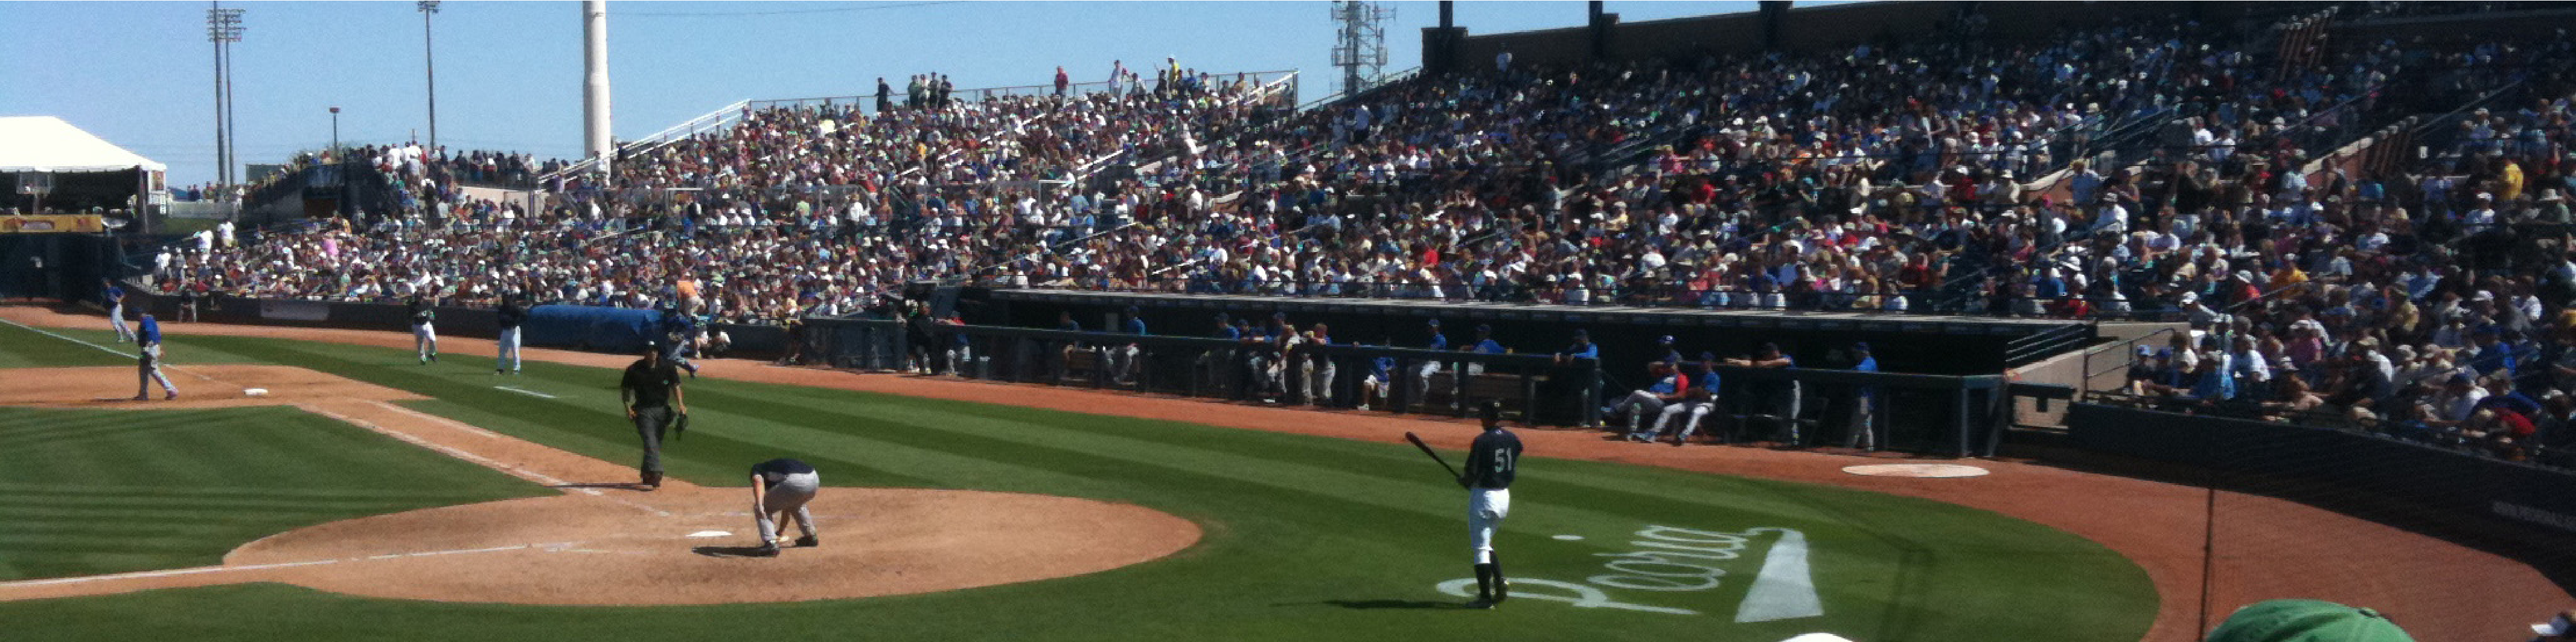
\includegraphics[width=\textwidth]{sampleteaser}
%  \caption{Seattle Mariners at Spring Training, 2010.}
%  \Description{Enjoying the baseball game from the third-base
%  seats. Ichiro Suzuki preparing to bat.}
%  \label{fig:teaser}
%\end{teaserfigure}

%%
%% This command processes the author and affiliation and title
%% information and builds the first part of the formatted document.
\maketitle

% Abstract
% Introduction
% Methodology
% Results
% Discussion
% Conclusion
% Recommendations.
\ifx\homepath\overleafhome
% Overleaf compilation.

% Include chapters.
%\begin{abstract}
  %Energy efficient applications of artificial intelligence (AI) may be able to increase space robot autonomy. 
  This research sets out to test whether principles of brain adaptation can be leveraged to increase the radiation resistance of neuromorphic space hardware. Neuromorphic architectures provide energy efficient platforms for AI applications in space. Structural similarities between neuromorphic architectures and the brain may allow them to benefit from brain-inspired design on the topic of damage recovery. Space environments can provide challenging conditions with significant radiation exposure, that may damage neuromorphic space hardware. A brain-inspired approach is explored in mitigating such damage.
  
  This approach is investigated using simulated radiation robustness tests with- and without brain adaptation implementation. The differences in radiation robustness are then analysed and discussed in the context of space applications of neuromorphic hardware. The SNN implementation by Diehl et al. of the minimum dominating set approximation algorithm by Alipour et al. is enhanced with brain adaptation mechanisms for these tests \cite{alipour2020distributed}\cite{diehl}. The tests are performed using Intel's Lava framework V0.3.0.
\end{abstract}
\chapter{Introduction}\label{chap:baseline_introduction}
This document presents the baseline for the AE5810 Thesis Project of the Space Flight Master at the Faculty of Aerospace Engineering of Delft University of Technology and the SOW-MKI92 Research Project of the Master in Artificial Intelligence at the faculty of Social Sciences of Radboud University. Its purpose is to identify the 2-5 most feasible design options that can be used to determine whether the principle of brain adaptation can be leveraged in neuromorphic space hardware.


The baseline report presents the \acrfull{ffd} and \acrfull{fbd} in \cref{chap:baseline_ffd} and \cref{chap:baseline_fbd} respectively. These function descriptions of the system that is to be designed, is then used to generate the \acrfull{rdt} in \cref{chap:baseline_requirements_discovery_tree}. Next, the resource allocation and budget breakdown presented in \cref{chap:baseline_resource_allocation_budget_breakdown}. This is followed by the technical risk assessment in \cref{chap:baseline_technical_risk_assessment}. From the \acrshort{rdt}, the \acrfull{dot} is generated in \cref{chap:baseline_requirements_discovery_tree}. Contingency management is applied in \cref{chap:baseline_contingency_management}. A market analysis is presented in \cref{chap:baseline_market_analysis}, and the sustainable development strategy is presented in \cref{chap:baseline_sustainable_development_management}. To ensure this work is performed with sufficient quality, the reporting and quality control is presented in \cref{chap:baseline_reporting_and_quality_control}. The baseline is concluded in \cref{chap:baseline_conclusion}.
\section{Brain Adaptation}\label{sec:brain_adaptation}
Four methods of brain adaptation have been explored within this research to find brain-inspired adaptation mechanisms; redundancy, reorganisation, niche construction and timing of developmental trajectories.  Starting with redundancy, it is noted that higher vertebrate brains often have multiple neural pathways that can support certain behaviour \cite{johnson_brain_2015}. Using multiple pathways is considered a viable strategy of implementing brain adaptation in the generated SNN. However, for completeness, reorganisation and niche construction are also evaluated. Continuing with reorganisation, evidence suggests that the human brain becomes increasingly hierarchical during post-natal development \cite{supekar_brain_2013}. No levels of hierarchy are found in the generated SNN. It is noted that for more advanced applications, such as on-site learning/retraining, the increases in hierarchy of the SNN might allow for automatic recovery after radiation exposure. An example could be a pre-trained network performing re-training after passing through the Van Allen belts before arriving at another solar body. Next, niche construction has been seen in some organisms that can change the neural pathways to select environment information based on a combination of which information the organism needs and what the brain can best process \cite{johnson_brain_2015}. It is expected that including the aspect of what the brain can best process requires a highly advanced combination of objective functions and information input streams. This option is not considered feasible within this research project. Timing of developmental trajectories can be seen as a compensation mechanism that delays the development of certain brain regions such that the brain can sample information from early environments such that it can optimise its development structure \cite{johnson_brain_2015}. The timing of developmental trajectories could be applied to a Mars rover that learns object detection on Mars instead of on Earth, using two different sensory inputs to provide input data and labels. If there are significant learnable differences with respect to the Earth environment, it could lead to a better trained model. In the context of the radiation robustness, the optimisation of the development structure could be used to ignore damaged neurons after radiation exposure. Redundancy is selected as the primary method of brain-adaptation for the selected SNN implementation of the MDS approximation algorithm because it does not require structural hierarchies nor model training.

To see how this redundancy can be implemented, the following neural coding mechanisms are evaluated:
\begin{itemize}
    \item \textit{Rate/frequency coding} - Assumes frequency or rate of action potential increases are accompanied by stimulus intensity increases.
    \item \textit{Temporal coding} - Uses high-frequency firing rate fluctuations to convey information. %Some natural frequency oscillations may be used to intelligently restructure the network using this concept.}
    \item \textit{Population coding} - Represents stimuli using combined activities of multiple neurons.% Work by fellow student Fabian Schneider at the Donders Institute showed this method in particular proved useful in the context of robustness SNNs. Fabian's work will be taken into account in the baseline, midterm and final phase where relevant.}
    \item \textit{Sparse coding} - Uses small subsets of neurons to encode items. %Perhaps this mechanism can be used at times to represent redundant information.}
\end{itemize}
Rate/frequency adjustments can be used to increase or lower the \textit{precision} % TODO: verify this is the correct word. 
of the spiking representation of numbers. By increasing the frequency, the relative impact of radiation induced spike omission could be reduced. % TODO: include proof of concept.
Similarly, with population coding, the population size adjustments can be used to lower the relative impact of radiation induced neuron deaths on numerical representation accuracies. No useful implementations for temporal coding and sparse coding are found in the context of radiation robustness of the generated SNN algorithm for the MDS approximation.

In order to increase the energy efficiency of the designed SNN implementation, a sparse coding scheme has been used. Single neurons and spikes are used to encode integers.
\section{Methodology}\label{sec:methodology}
The research methodology starts in \cref{subsec:algorithm} with a description of the minimum dominating set (MDS) approximation algorithm by Alipour, the SNN implementation of this algorithm by Diehl et al., and the implemented form %TODO: form or forms? 
of brain adaptation \cite{alipour2020distributed}\cite{diehl}. Since the overarching research project aims at performing physical radiation tests, \cref{subsec:hardware} specifies the hardware that is used for testing, and how the radiation effects are simulated. The test procedure is detailed in \cref{subsec:testing}.

\subsection{Algorithm Selection}\label{subsec:algorithm}
The MDS approximation as presented by Alipour et al., is specified in Alg. 1.
%Within the graph algorithms, some SNN algorithms may be naturally more robust than others. For example, SNN algorithms that calculate the shortest path within graphs may automatically re-route if radiation imposed neuron-death occurs. However, since this research aims at determining the effectivity of brain adaptation mechanisms, a stricter test is found in algorithms that can fail to produce meaningful output if a single neuronal or synaptic property is changed. Therefore, 
\begin{algorithm}[h]%[1]
    \caption{Distributed Algorithm for computing a total dominating set in a graph with given integer $m\geq 0$.}\label{alg:alipour}
    \KwData{Connected, planar, triangle-free graph of size $n$.}
    \KwResult{Set of nodes that form a minimum total dominating set (MDTS).}
    In the first round, each node $v_i$ chooses a random number $0<r_i<1$ and computes its weight $w_i=d_i+r_i$ and sends $w_i$ to its
    adjacent neighbours.\;
    In the second round, each node $v$ marks a neighbour vertex $v_i$ whose weight $w_i$ is maximum among all the other neighbours of $v$.\;
    \For{$m$ rounds}{
        Let $x_i$ be the number of times that a vertex is marked by its neighbour vertices, let $w_i=x_i+r_i$\;
        Unmark the marked vertices.\;
        Each vertex marks the vertex with maximum $w_i$ among its neighbour vertices.\;
    }
    8: The marked vertices are considered as the vertices in our total dominating set for $G$.\;
\end{algorithm}
Next, an SNN implementation of this algorithm is generated using Leaky-Integrate-and-Fire (LIF) neurons. This implementation is created by Diehl et al. \cite{diehl} using the open-source Lava software framework by Intel. This implementation takes as input connected, triangle-free, planar graphs (E.g. \cref{fig:input_graph}). Then it converts these graphs into the specification of an SNN that is encoded in a new graph (E.g. \cref{fig:encoded_snn}). A recursive method then takes a single neuron and converts the encoded SNN that is encoded in the graph into an actual functional SNN that can be run on the simulated on a regular computer.
\begin{figure}[]
    \centering
    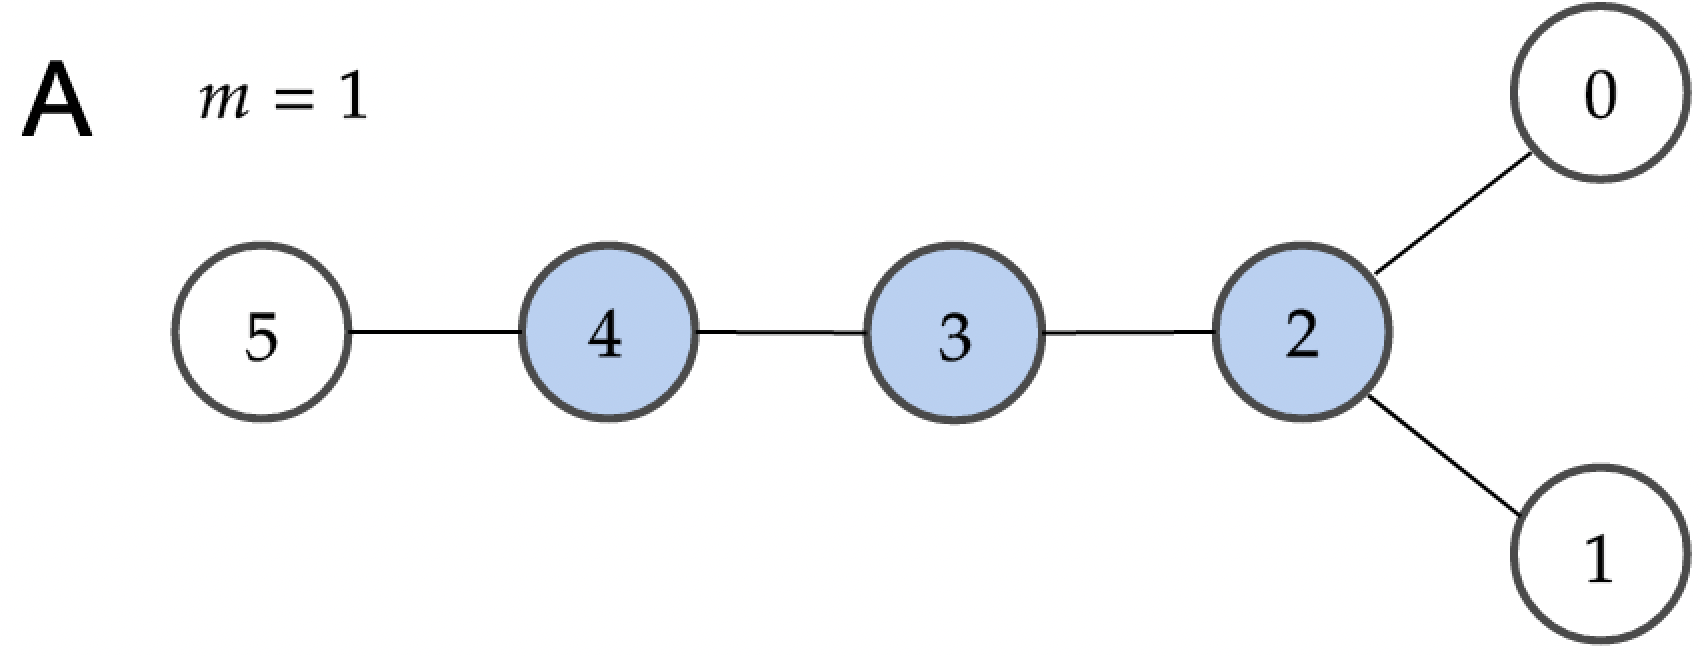
\includegraphics[width=8cm]{latex/Images/input_graph_G_6_0_alternative1.png}
    \caption{Example input graph. For $m=1$ the algorithm still selects 3 nodes as it is an approximation of the MDS.}
    \label{fig:input_graph}
\end{figure}

\begin{figure}[]
    \centering
    %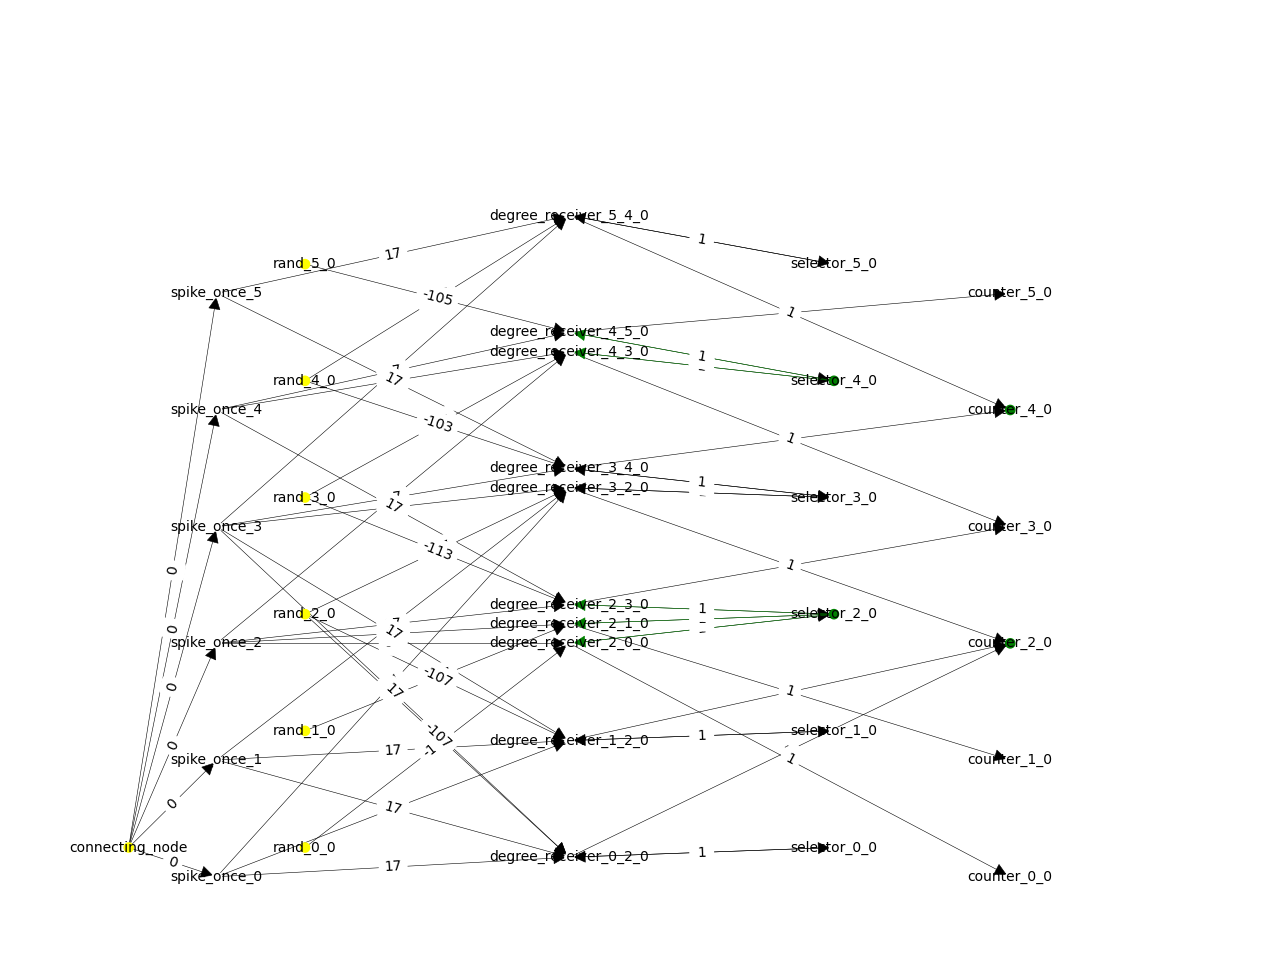
\includegraphics[width=8cm]{latex/Images/structured_graph_snn_m0_n6_iter0_t77.png}
    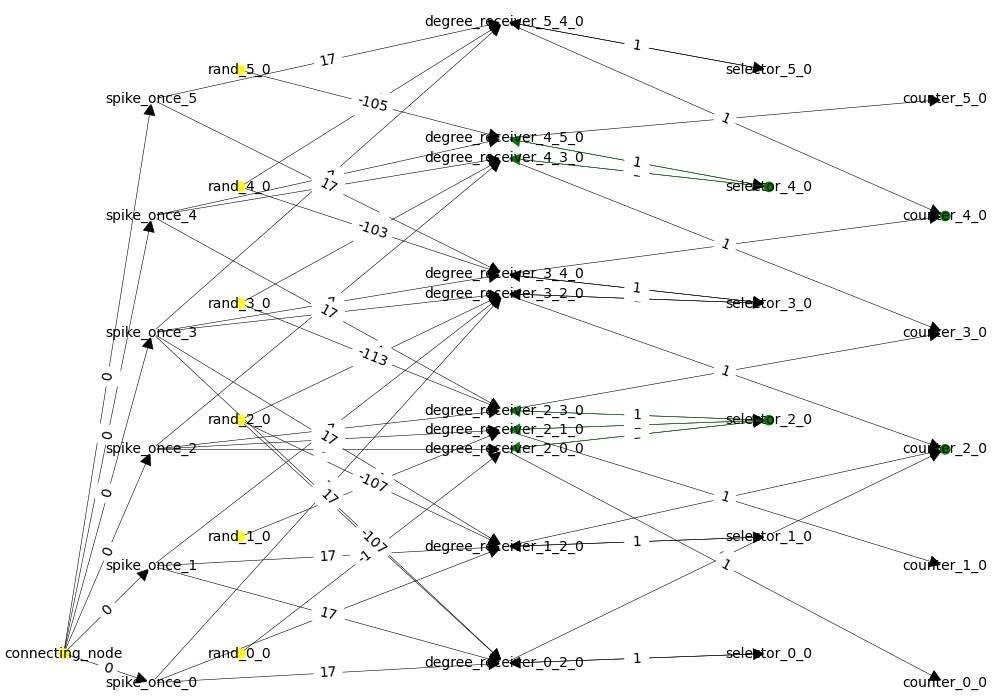
\includegraphics[width=\linewidth]{latex/Images/cropped.jpeg}
    \caption{Example SNN encoding of algorithm to approximate MDS on the input graph of \cref{fig:input_graph}. This module is connected in series where the mark counter neuron takes up the role of spike\_once neuron in the next round of the approximation algorithm. For a more detailed description of the SNN implementation the reader is referred to Diehl et al. \cite{diehl}. %TODO: update to match updated input graph.
    }
    \label{fig:encoded_snn}
\end{figure}

\noindent This SSN implementation of the MDS approximation algorithm is onwards referred to as the default network. This default network is enhanced with strategically placed redundant neurons that are inhibited by the default network neurons. Next, space radiation damage is simulated on the Loihi 2 in the form of random neuron deaths. These neuron deaths imply that a neuron is removed from the SNN, which can occur in both the default network and the set of redundancy neurons. If a default network neuron dies, the inhibition to the redundant neuron should be removed, causing the SNN to use the alternative neural pathway to recover from this damage. This usage of the alternative neural pathway simulates the multi-pathway structures found in brains of higher vertebrates and is proposed as the main adaptive mechanism in response to damage.

\subsection{Hardware}\label{subsec:hardware}
At the time of writing, no single-event effect (SEEs) propagation mechanisms are identified for space radiation exposure on the Loihi 1 \& 2  neuromorphic chips, a high-level software simulation of these single-event effects is performed. This is done by assuming that the non-neuromorphic components of the chips are performing nominally, and that the SEEs propagate from, for example, transient bit-flips, towards neuronal and synaptic parameter changes. The first assumptions may be accurate if local radiation hardening and redundancy is applied to the non-neuromorphic components. Weight and/or energy saving could be a motivation to apply these radiation counter-measures sparsely. The second assumption is based on the digital nature of the components that make up the neural components of the Loihi. The components that make up the neural compartments and synapses of the Loihi are visualised in \cref{fig:loihi_micro_architecture}.
\begin{figure}[H]
    \centering
    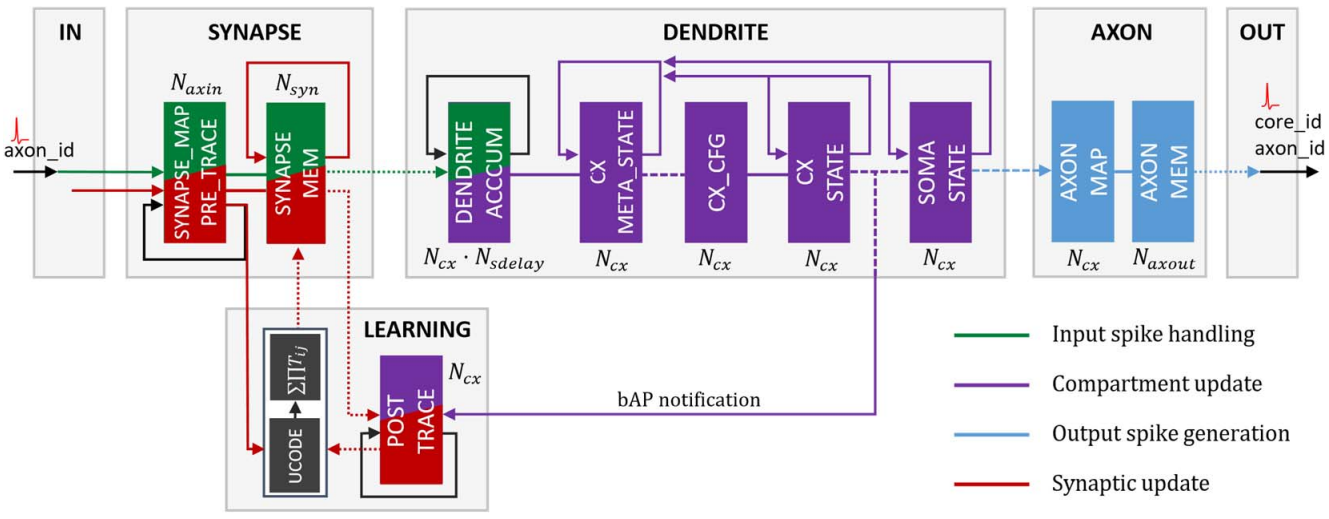
\includegraphics[width=8cm]{latex/Images/loihi_micro_architecture.png}
    \caption{Core Top-Level Microarchitecture of the Loihi chip. The SYNAPSE unit processes all incoming spikes and
    reads out the associated synaptic weights from the SRAM memory \cite{davies_loihi_2018}
    .}
    \label{fig:loihi_micro_architecture}
\end{figure}



\subsection{Testing}\label{subsec:testing}
To test whether the brain adaptation implementation may be used to increase radiation robustness of neuromorphic space hardware, it is compared to a baseline without brain adaptation. 

% TODO: verify subsubsections are allowed.
\subsubsection{Metrics}\label{subsubsec:metrics}
The metrics of the comparison are:
\begin{enumerate}
    \item \textit{Radiation Robustness} - a percentage score indicating the ratio of successful solution generation on random input graphs.
    \item \textit{Neuronal \& Synaptic Overcapacity} - a factor from 0 to $n$, indicating the ratio of redundant neurons and synapses with respect to the original implementation without adaptation implementation. % TODO: consistent default network naming see method/intro.
    \item \textit{Energy Efficiency} - the number of spikes consumed by implementations.
    %\item \textit{Time complexity} - the theoretical time complexity required for network initialisation and adaptation.
    %\item \textit{Space Complexity} - the theoretical space complexity required for network initialisation and adaptation.
\end{enumerate}

\subsubsection{Simulated Radiation Damage}\label{subsubsec:simulated_radiation_damage}
This work simulates radiation damage propagation of SEEs as neuron deaths by setting the neuron thresholds $vth=1000 [V]$ at from the start of the simulation. The 1000 [V] is arbitrary yet large enough to prevent spiking. Transient effects are ignored along with neuron property changes in $\delta u,\delta v, bias$, synaptic death, and synaptic property changes in: $sign,weight$.

\subsubsection{Brain Adaptation Mechanism}\label{subsubsec:brain_adaptation_mechanisms}
The selected SNN implementation is enhanced with redundant neurons and neuronal pathways to realise simulated radiation robustness. A basic example is shown in \cref{fig:eg_brain_adaptation}.
\begin{figure}[H]
    \centering
    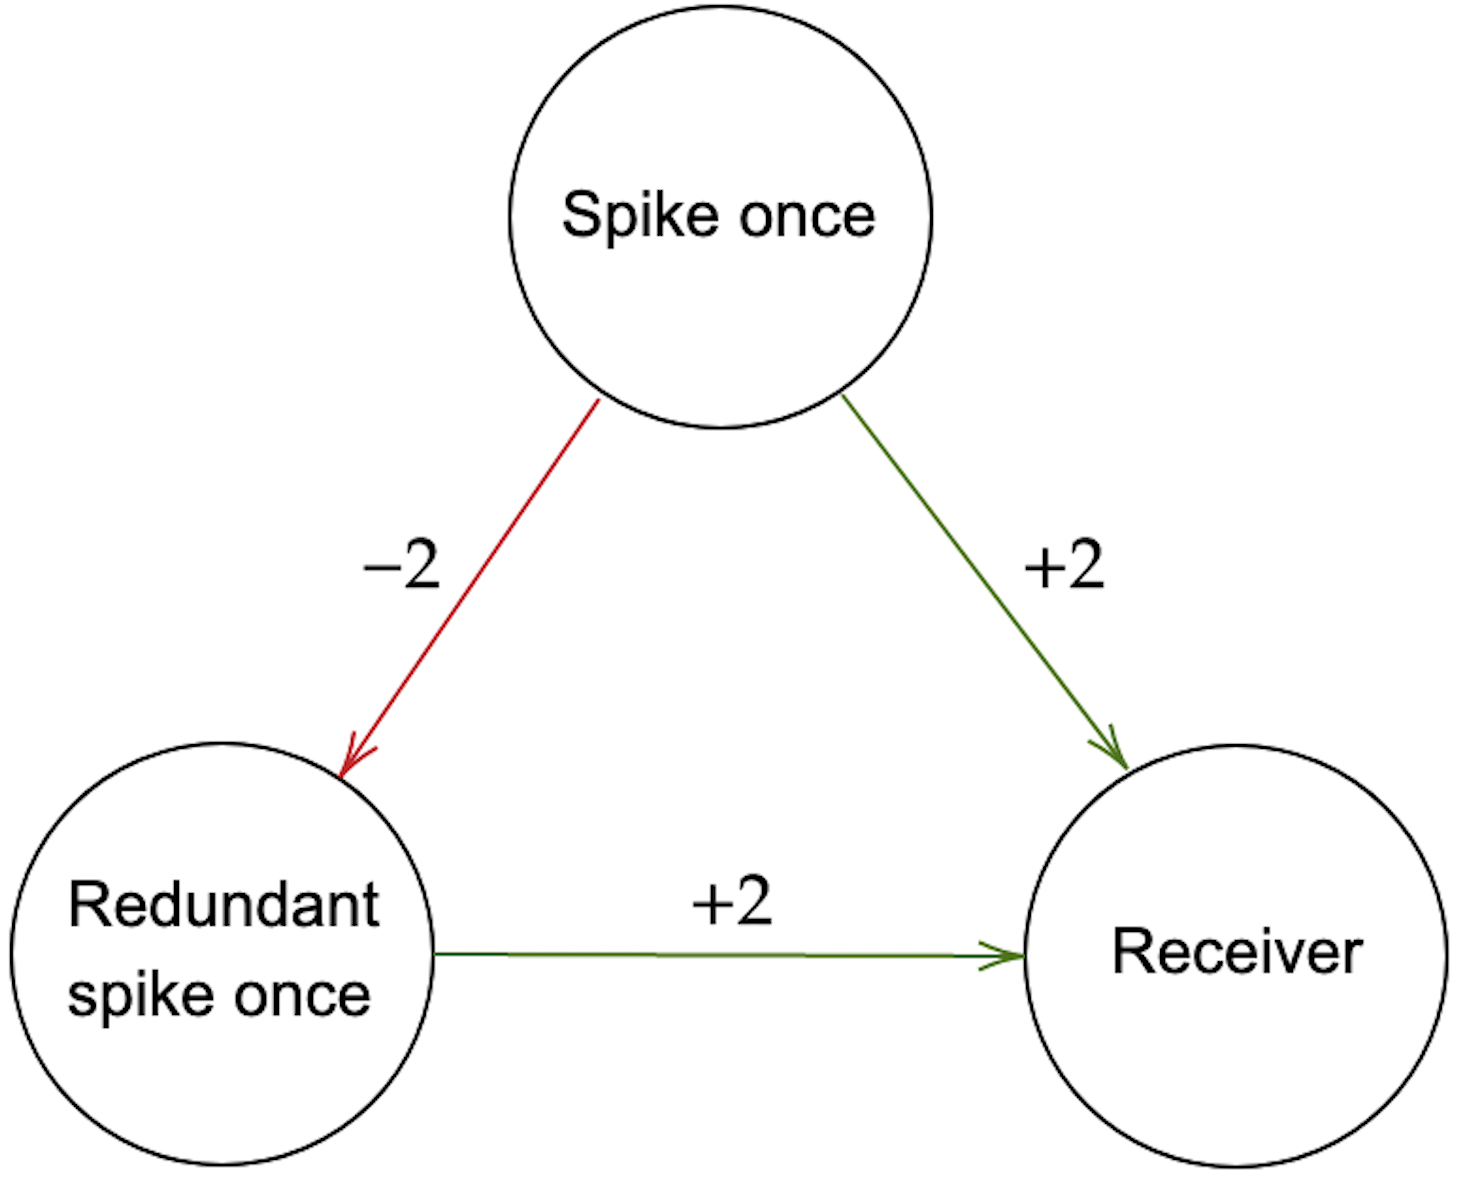
\includegraphics[width=.5\linewidth]{latex/Images/brain_adaptation_alternative.png}
    \caption{Alternative neural pathway for a redundancy of the spike\_once neuron. If the spike\_once neuron dies due to simulated radiation-induced SEEs ($vth=inf$), the redundancy neuron inhibition is eliminated. Without inhibition, the redundant spike\_once neuron copies the spike\_once behaviour with a delay of 1 timestep.}
    \label{fig:eg_brain_adaptation}
\end{figure}

\noindent The alternative neural pathway renders a single neuron $original_i$ with $a$ input synapses, and $b$ output synapses, redundant at the cost of $2a+2b$ synapses and 2 neurons. This cost can be reduced by implementing a controller that scans the network and manually redirects neural pathways to a smaller buffer network. However, that shifts the radiation robustness problem as that controller may also endure SEEs. % This does allow local shielding to be used, and may use components that are physically more robust than the SNN networks.
One can also add triple/$n$-factor redundancy by including more redundant spike\_once neurons that are inhibited by the original spike\_once neuron and each other. This induces an additional delay of t=1 time step per redundant neuron.

%\item \textcolor{red}{An Neumann monitoring module that scans the entire SNN network probing its behaviour, and re-routing broken neurons and/or synapses to redundant neurons.}
%\item \textcolor{red}{A rate-coding frequency adaptation to reduce the relative impact of radiation induced spike omission in a subnetwork of the complete SNN implementation of the MDS approximation.}

\section{Results}\label{sec:results}
%The domains specified in \cref{subsec:results_energy_consumption} to \cref{subsec:results_radiation_robustness} are evaluated as part of the presentation of the results of this experiment. The first three are used to put the radiation robustness in perspective. All four domains are compared to the reference baseline presented in \cref{sec:methodology}.

\subsection{Energy Consumption}\label{subsec:results_energy_consumption}
Barchart here: x-axis: radiation death percentage, per x-coordinate, 3 bars: 10\%,100\%,200\% redundancy, y-axis: percentage of correctly evaluated graphs.

If if multiple 
%\textit{Depending on the radiation test method, the energy consumption may be monitored hardwarematically, or estimated softwarematically. This may be challenging in the case of reliance on neuromorphic cloud architectures for testing, as some may not provide the ability to measure and/or report energy consumption. An approximation to the energy consumption could be counting the occurrence of neuron spikes. This is because neuromorphic architectures are considered to only consume significant amounts of energy when they spike.}

\subsection{Neuronal \& Synaptic Overcapacity}\label{subsec:results_neuronal_synaptic_overcapacity}
By taking this factor into account, a context can be provided for the added value of using brain-inspired radiation robustness implementations in neuromorphic hardware.

\subsection{Traditional Hardware Element Performance}\label{subsec:results_traditional_hardware_element_performance}
\textit{Typical neuromorphic hardware still contains some traditional/Von Neumann architecture components, such as a memory bus and processor. These are typically used to communicate with the outside world, and to orchestrate/set up/initialise the neural network \cite{todo}. Given this position high in the functional hierarchy, they may form a critical bottleneck in terms of radiation robustness. To overcome this issue, a recommendation could be included to increase the shielding and/or redundancy of these Von Neumann components, whilst saving mass and redundancy in the spiking neural networks using brain-inspired implementations \cite{johan_kwisthout_personal_corrospondence_feb_15}.}

\subsection{Radiation Robustness}\label{subsec:results_radiation_robustness}
\textit{This section will be used to present the radiation robustness of the tested neuromorphic architectures with- and without brain-inspired implementation.}
\section{Discussion}\label{sec:discussion}
The reliability of the results can be improved by increasing running the algorithm on more and larger graphs. Running on the Loihi 2 using the Lava 0.4.0 Framework may facilitate this. Even though no public SEE propagation mechanisms are known for the Loihi 2 at the time of writing, the representativeness of the simulation can be increased by taking transient effects, synaptic changes, neuron property changes and Von Neumann component malfunctions into account. The current form of redundancy that is implemented is still dependent on particular neuron properties, and no automated method for arbitrary LIF neuron redundancy is presented. A more intelligent adaptation mechanism may allow for a more active neural pathway redirection to realise equivalent robustness levels at a lower neuronal and synaptic overhead. 
%The discussion is used to put the/any radiation robustness differences between using a brain-inspired implementation and regular redundancy in neuromorphic architectures, into perspective. This perspective is generated by discussing the architecture comparison in terms of the characteristics described in \cref{subsec:discussion_performance_trade_off} to \cref{subsec:discussion_space_application_representation_accuracy}.

%\subsection{Performance Trade-Off}\label{subsec:discussion_performance_trade_off}
%\textit{Increasing the radiation resistance of a default neuromorphic implementation requires some effort. In this study, this effort is realised in the form of a brain-inspired implementation. Such an implementation comes at the cost of resources. In this case those resources are neurons, synapses and energy consumption. Since the comparison is made in terms of radiation robustness, it is important to determine whether it is not merely the consumption of extra resources that led to performance differences. In particular, for space applications, it is important to determine whether the resources that are consumed, for example the energy consumption, are worth the benefits. Each space mission will have its own trade-off in these terms, however, this subsection can shed some light on the trade-off costs. In essence a quantitative insight can be given in terms of performance enhancement and energy cost increases. Similarly, a quantitative insight can be provided in terms of performance enhancement, and the increase in required neurons/synapses and/or hardware mass (if the increase in neurons/synapses require a larger chip).}

%\subsection{Simulation vs Radiation Testing}
%\textit{If the radiation testing is performed softwarematically in this article submission, this section can be used to convey how portable these results are expected to be to practical radiation tests.}

%\subsection{Radiation Robustness of Traditional Hardware Elements}
%\textit{The potential bottleneck of traditional Von Neumann hardware elements in neuromorphic hardware, as introduced in \cref{subsec:results_traditional_hardware_element_performance} should be discussed in this section.}

%\subsection{Space Application Representation Accuracy}\label{subsec:discussion_space_application_representation_accuracy}
%\textit{Some context can be provided in this section to indicate how/up to what extent the radiation testing that is performed for this article submission applies to real space applications.}
% Explain actual space applications may be more AI and less optimisation.
\section{Conclusion}\label{sec:conclusion}
% Talk about results.
%The results presented in \cref{sec:results}, along with their critical context described in \cref{sec:discussion} are to be synthesised in this section to provide a clear insight into the benefits and drawbacks of leveraging implementations inspired by principles of brain adaptation in neuromorphic hardware to increase the radiation robustness of these architectures in space applications.
% Talk about discussion
% Mention whether or not it helped.
Brain-inspired adaptation mechanisms may be used in SNN implementations of graph optimisation problems to increase the radiation robustness of neuromorphic space hardware if SEE propagations can lead to neuron death. Creating more intelligent adaptation mechanisms than separate redundant neuronal pathways for each neuron may improve the radiation results at a lower neuronal overhead. 

% Don't mention that symmetries in distributed algorithms may also be leveraged in lowering the cost of these brain adaptations. Not a conclusion, not mentioned before, not related to this work.

% TODO: write something about overhead and spike energy.
\section{Future Work}\label{sec:recommendations}
%\textit{Recommendations may be generated based on the listed issues in \cref{sec:discussion}. It is foreseeable that dedicated shielding and or redundancy of critical elements of traditional Von Neumann elements in neuromorphic architectures may be advisable, whilst relying on the brain-inspired implementations in SNNs. Another recommendation that may flow out of this research may concern the integration of brain adaptation principles into the design of SNN implementations that yield space application functionalities. Furthermore, a recommendation may be generated regarding a proposed shift in the moment of training, from pre-trained on the ground, to (re-)training after radiation exposure.}

The overarching research project aims to perform physical radiation tests to gain more insight in the practical usefulness of brain-inspired adaptation mechanisms to hedge against radiation damage in neuromorphic space hardware. Since these tests are costly, a more thorough analysis on a broader scope of adaptation mechanisms is proposed. In particular, the population coding and rate coding options will be explored, and the focus is shifted to more AI oriented applications. \cref{subsec:algorithm_selection} to  \cref{subsec:physical_testing}. 





%\input{chapters/7_acknowledgements.tex}
\else
% Local compilation

% Include chapters.
%\begin{abstract}
  %Energy efficient applications of artificial intelligence (AI) may be able to increase space robot autonomy. 
  This research sets out to test whether principles of brain adaptation can be leveraged to increase the radiation resistance of neuromorphic space hardware. Neuromorphic architectures provide energy efficient platforms for AI applications in space. Structural similarities between neuromorphic architectures and the brain may allow them to benefit from brain-inspired design on the topic of damage recovery. Space environments can provide challenging conditions with significant radiation exposure, that may damage neuromorphic space hardware. A brain-inspired approach is explored in mitigating such damage.
  
  This approach is investigated using simulated radiation robustness tests with- and without brain adaptation implementation. The differences in radiation robustness are then analysed and discussed in the context of space applications of neuromorphic hardware. The SNN implementation by Diehl et al. of the minimum dominating set approximation algorithm by Alipour et al. is enhanced with brain adaptation mechanisms for these tests \cite{alipour2020distributed}\cite{diehl}. The tests are performed using Intel's Lava framework V0.3.0.
\end{abstract}
\chapter{Introduction}\label{chap:baseline_introduction}
This document presents the baseline for the AE5810 Thesis Project of the Space Flight Master at the Faculty of Aerospace Engineering of Delft University of Technology and the SOW-MKI92 Research Project of the Master in Artificial Intelligence at the faculty of Social Sciences of Radboud University. Its purpose is to identify the 2-5 most feasible design options that can be used to determine whether the principle of brain adaptation can be leveraged in neuromorphic space hardware.


The baseline report presents the \acrfull{ffd} and \acrfull{fbd} in \cref{chap:baseline_ffd} and \cref{chap:baseline_fbd} respectively. These function descriptions of the system that is to be designed, is then used to generate the \acrfull{rdt} in \cref{chap:baseline_requirements_discovery_tree}. Next, the resource allocation and budget breakdown presented in \cref{chap:baseline_resource_allocation_budget_breakdown}. This is followed by the technical risk assessment in \cref{chap:baseline_technical_risk_assessment}. From the \acrshort{rdt}, the \acrfull{dot} is generated in \cref{chap:baseline_requirements_discovery_tree}. Contingency management is applied in \cref{chap:baseline_contingency_management}. A market analysis is presented in \cref{chap:baseline_market_analysis}, and the sustainable development strategy is presented in \cref{chap:baseline_sustainable_development_management}. To ensure this work is performed with sufficient quality, the reporting and quality control is presented in \cref{chap:baseline_reporting_and_quality_control}. The baseline is concluded in \cref{chap:baseline_conclusion}.
\section{Brain Adaptation}\label{sec:brain_adaptation}
Four methods of brain adaptation have been explored within this research to find brain-inspired adaptation mechanisms; redundancy, reorganisation, niche construction and timing of developmental trajectories.  Starting with redundancy, it is noted that higher vertebrate brains often have multiple neural pathways that can support certain behaviour \cite{johnson_brain_2015}. Using multiple pathways is considered a viable strategy of implementing brain adaptation in the generated SNN. However, for completeness, reorganisation and niche construction are also evaluated. Continuing with reorganisation, evidence suggests that the human brain becomes increasingly hierarchical during post-natal development \cite{supekar_brain_2013}. No levels of hierarchy are found in the generated SNN. It is noted that for more advanced applications, such as on-site learning/retraining, the increases in hierarchy of the SNN might allow for automatic recovery after radiation exposure. An example could be a pre-trained network performing re-training after passing through the Van Allen belts before arriving at another solar body. Next, niche construction has been seen in some organisms that can change the neural pathways to select environment information based on a combination of which information the organism needs and what the brain can best process \cite{johnson_brain_2015}. It is expected that including the aspect of what the brain can best process requires a highly advanced combination of objective functions and information input streams. This option is not considered feasible within this research project. Timing of developmental trajectories can be seen as a compensation mechanism that delays the development of certain brain regions such that the brain can sample information from early environments such that it can optimise its development structure \cite{johnson_brain_2015}. The timing of developmental trajectories could be applied to a Mars rover that learns object detection on Mars instead of on Earth, using two different sensory inputs to provide input data and labels. If there are significant learnable differences with respect to the Earth environment, it could lead to a better trained model. In the context of the radiation robustness, the optimisation of the development structure could be used to ignore damaged neurons after radiation exposure. Redundancy is selected as the primary method of brain-adaptation for the selected SNN implementation of the MDS approximation algorithm because it does not require structural hierarchies nor model training.

To see how this redundancy can be implemented, the following neural coding mechanisms are evaluated:
\begin{itemize}
    \item \textit{Rate/frequency coding} - Assumes frequency or rate of action potential increases are accompanied by stimulus intensity increases.
    \item \textit{Temporal coding} - Uses high-frequency firing rate fluctuations to convey information. %Some natural frequency oscillations may be used to intelligently restructure the network using this concept.}
    \item \textit{Population coding} - Represents stimuli using combined activities of multiple neurons.% Work by fellow student Fabian Schneider at the Donders Institute showed this method in particular proved useful in the context of robustness SNNs. Fabian's work will be taken into account in the baseline, midterm and final phase where relevant.}
    \item \textit{Sparse coding} - Uses small subsets of neurons to encode items. %Perhaps this mechanism can be used at times to represent redundant information.}
\end{itemize}
Rate/frequency adjustments can be used to increase or lower the \textit{precision} % TODO: verify this is the correct word. 
of the spiking representation of numbers. By increasing the frequency, the relative impact of radiation induced spike omission could be reduced. % TODO: include proof of concept.
Similarly, with population coding, the population size adjustments can be used to lower the relative impact of radiation induced neuron deaths on numerical representation accuracies. No useful implementations for temporal coding and sparse coding are found in the context of radiation robustness of the generated SNN algorithm for the MDS approximation.

In order to increase the energy efficiency of the designed SNN implementation, a sparse coding scheme has been used. Single neurons and spikes are used to encode integers.
\section{Methodology}\label{sec:methodology}
The research methodology starts in \cref{subsec:algorithm} with a description of the minimum dominating set (MDS) approximation algorithm by Alipour, the SNN implementation of this algorithm by Diehl et al., and the implemented form %TODO: form or forms? 
of brain adaptation \cite{alipour2020distributed}\cite{diehl}. Since the overarching research project aims at performing physical radiation tests, \cref{subsec:hardware} specifies the hardware that is used for testing, and how the radiation effects are simulated. The test procedure is detailed in \cref{subsec:testing}.

\subsection{Algorithm Selection}\label{subsec:algorithm}
The MDS approximation as presented by Alipour et al., is specified in Alg. 1.
%Within the graph algorithms, some SNN algorithms may be naturally more robust than others. For example, SNN algorithms that calculate the shortest path within graphs may automatically re-route if radiation imposed neuron-death occurs. However, since this research aims at determining the effectivity of brain adaptation mechanisms, a stricter test is found in algorithms that can fail to produce meaningful output if a single neuronal or synaptic property is changed. Therefore, 
\begin{algorithm}[h]%[1]
    \caption{Distributed Algorithm for computing a total dominating set in a graph with given integer $m\geq 0$.}\label{alg:alipour}
    \KwData{Connected, planar, triangle-free graph of size $n$.}
    \KwResult{Set of nodes that form a minimum total dominating set (MDTS).}
    In the first round, each node $v_i$ chooses a random number $0<r_i<1$ and computes its weight $w_i=d_i+r_i$ and sends $w_i$ to its
    adjacent neighbours.\;
    In the second round, each node $v$ marks a neighbour vertex $v_i$ whose weight $w_i$ is maximum among all the other neighbours of $v$.\;
    \For{$m$ rounds}{
        Let $x_i$ be the number of times that a vertex is marked by its neighbour vertices, let $w_i=x_i+r_i$\;
        Unmark the marked vertices.\;
        Each vertex marks the vertex with maximum $w_i$ among its neighbour vertices.\;
    }
    8: The marked vertices are considered as the vertices in our total dominating set for $G$.\;
\end{algorithm}
Next, an SNN implementation of this algorithm is generated using Leaky-Integrate-and-Fire (LIF) neurons. This implementation is created by Diehl et al. \cite{diehl} using the open-source Lava software framework by Intel. This implementation takes as input connected, triangle-free, planar graphs (E.g. \cref{fig:input_graph}). Then it converts these graphs into the specification of an SNN that is encoded in a new graph (E.g. \cref{fig:encoded_snn}). A recursive method then takes a single neuron and converts the encoded SNN that is encoded in the graph into an actual functional SNN that can be run on the simulated on a regular computer.
\begin{figure}[]
    \centering
    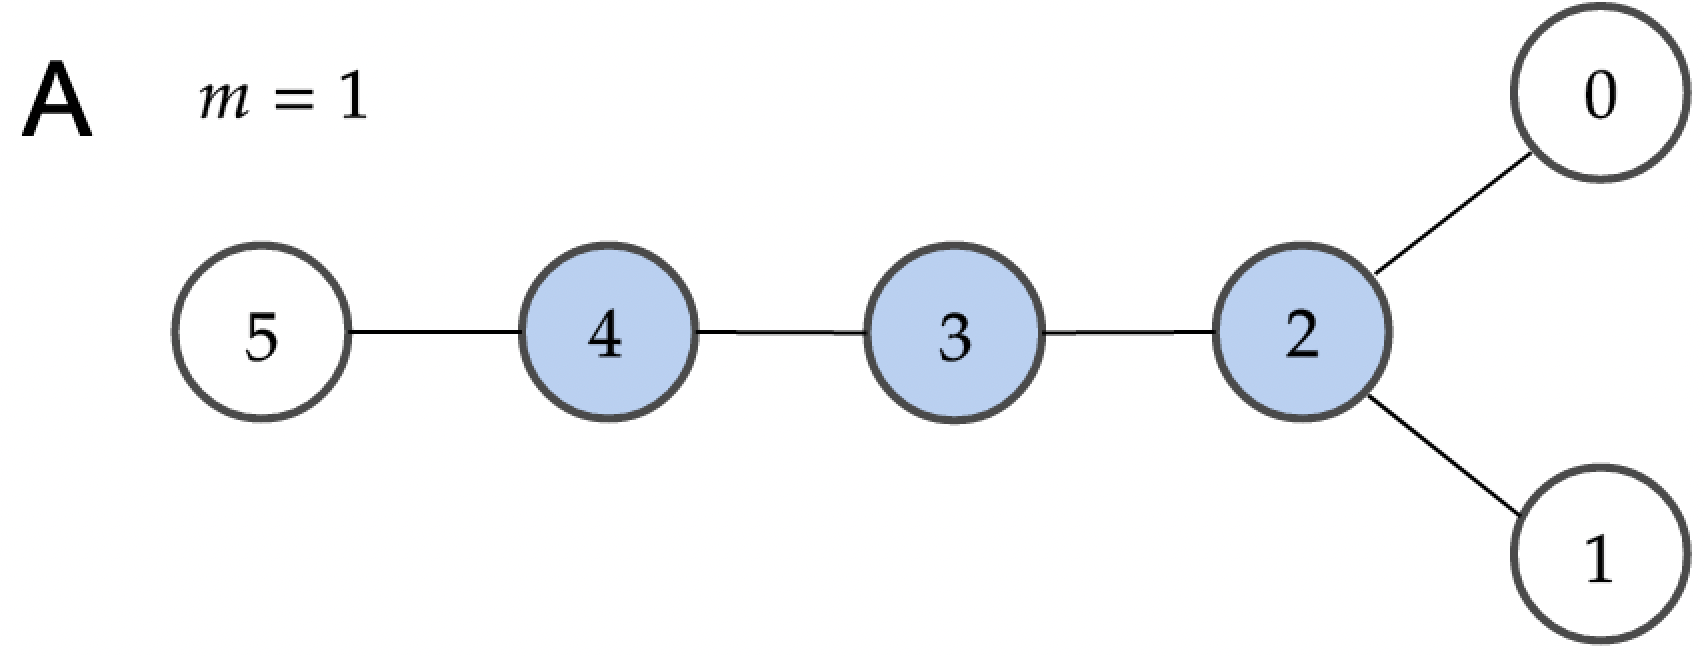
\includegraphics[width=8cm]{latex/Images/input_graph_G_6_0_alternative1.png}
    \caption{Example input graph. For $m=1$ the algorithm still selects 3 nodes as it is an approximation of the MDS.}
    \label{fig:input_graph}
\end{figure}

\begin{figure}[]
    \centering
    %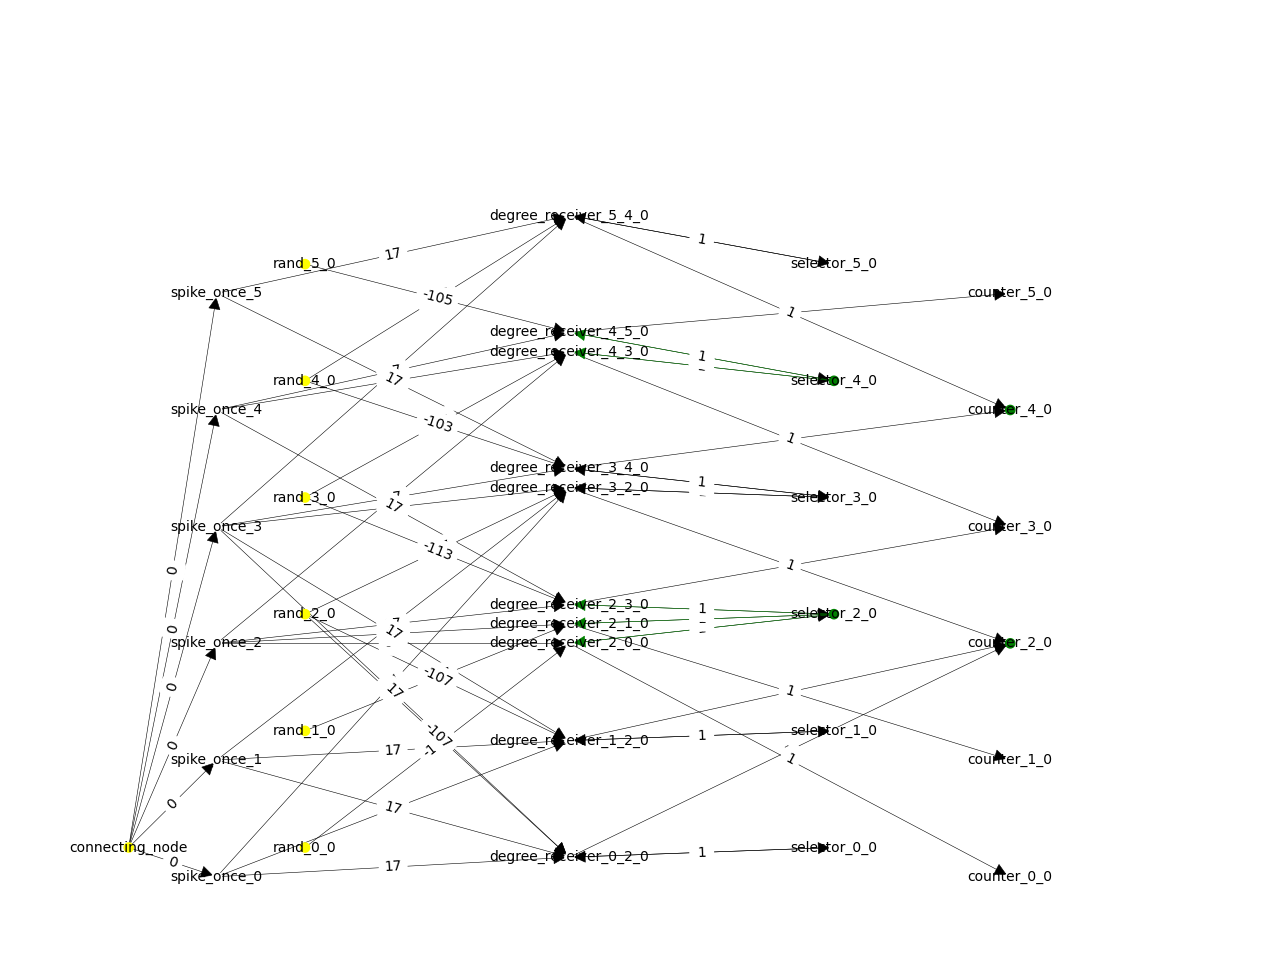
\includegraphics[width=8cm]{latex/Images/structured_graph_snn_m0_n6_iter0_t77.png}
    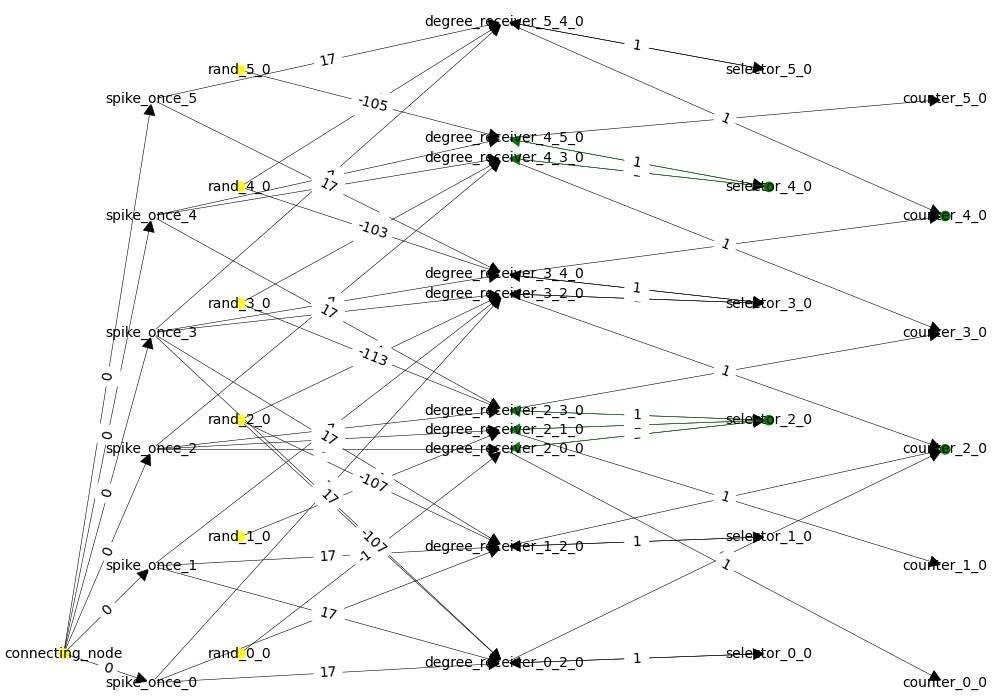
\includegraphics[width=\linewidth]{latex/Images/cropped.jpeg}
    \caption{Example SNN encoding of algorithm to approximate MDS on the input graph of \cref{fig:input_graph}. This module is connected in series where the mark counter neuron takes up the role of spike\_once neuron in the next round of the approximation algorithm. For a more detailed description of the SNN implementation the reader is referred to Diehl et al. \cite{diehl}. %TODO: update to match updated input graph.
    }
    \label{fig:encoded_snn}
\end{figure}

\noindent This SSN implementation of the MDS approximation algorithm is onwards referred to as the default network. This default network is enhanced with strategically placed redundant neurons that are inhibited by the default network neurons. Next, space radiation damage is simulated on the Loihi 2 in the form of random neuron deaths. These neuron deaths imply that a neuron is removed from the SNN, which can occur in both the default network and the set of redundancy neurons. If a default network neuron dies, the inhibition to the redundant neuron should be removed, causing the SNN to use the alternative neural pathway to recover from this damage. This usage of the alternative neural pathway simulates the multi-pathway structures found in brains of higher vertebrates and is proposed as the main adaptive mechanism in response to damage.

\subsection{Hardware}\label{subsec:hardware}
At the time of writing, no single-event effect (SEEs) propagation mechanisms are identified for space radiation exposure on the Loihi 1 \& 2  neuromorphic chips, a high-level software simulation of these single-event effects is performed. This is done by assuming that the non-neuromorphic components of the chips are performing nominally, and that the SEEs propagate from, for example, transient bit-flips, towards neuronal and synaptic parameter changes. The first assumptions may be accurate if local radiation hardening and redundancy is applied to the non-neuromorphic components. Weight and/or energy saving could be a motivation to apply these radiation counter-measures sparsely. The second assumption is based on the digital nature of the components that make up the neural components of the Loihi. The components that make up the neural compartments and synapses of the Loihi are visualised in \cref{fig:loihi_micro_architecture}.
\begin{figure}[H]
    \centering
    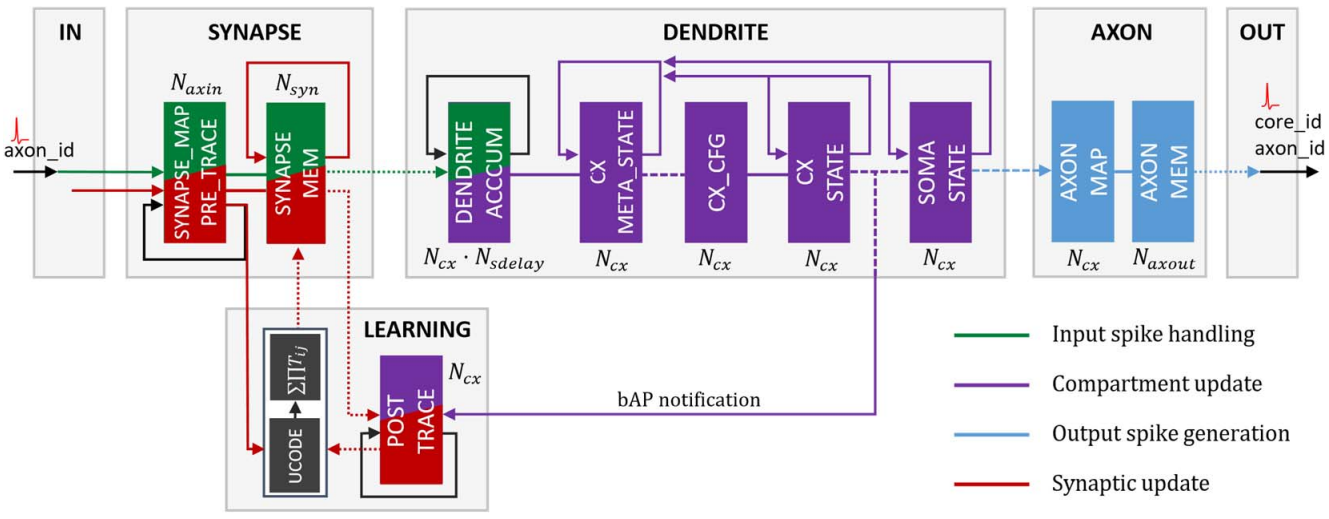
\includegraphics[width=8cm]{latex/Images/loihi_micro_architecture.png}
    \caption{Core Top-Level Microarchitecture of the Loihi chip. The SYNAPSE unit processes all incoming spikes and
    reads out the associated synaptic weights from the SRAM memory \cite{davies_loihi_2018}
    .}
    \label{fig:loihi_micro_architecture}
\end{figure}



\subsection{Testing}\label{subsec:testing}
To test whether the brain adaptation implementation may be used to increase radiation robustness of neuromorphic space hardware, it is compared to a baseline without brain adaptation. 

% TODO: verify subsubsections are allowed.
\subsubsection{Metrics}\label{subsubsec:metrics}
The metrics of the comparison are:
\begin{enumerate}
    \item \textit{Radiation Robustness} - a percentage score indicating the ratio of successful solution generation on random input graphs.
    \item \textit{Neuronal \& Synaptic Overcapacity} - a factor from 0 to $n$, indicating the ratio of redundant neurons and synapses with respect to the original implementation without adaptation implementation. % TODO: consistent default network naming see method/intro.
    \item \textit{Energy Efficiency} - the number of spikes consumed by implementations.
    %\item \textit{Time complexity} - the theoretical time complexity required for network initialisation and adaptation.
    %\item \textit{Space Complexity} - the theoretical space complexity required for network initialisation and adaptation.
\end{enumerate}

\subsubsection{Simulated Radiation Damage}\label{subsubsec:simulated_radiation_damage}
This work simulates radiation damage propagation of SEEs as neuron deaths by setting the neuron thresholds $vth=1000 [V]$ at from the start of the simulation. The 1000 [V] is arbitrary yet large enough to prevent spiking. Transient effects are ignored along with neuron property changes in $\delta u,\delta v, bias$, synaptic death, and synaptic property changes in: $sign,weight$.

\subsubsection{Brain Adaptation Mechanism}\label{subsubsec:brain_adaptation_mechanisms}
The selected SNN implementation is enhanced with redundant neurons and neuronal pathways to realise simulated radiation robustness. A basic example is shown in \cref{fig:eg_brain_adaptation}.
\begin{figure}[H]
    \centering
    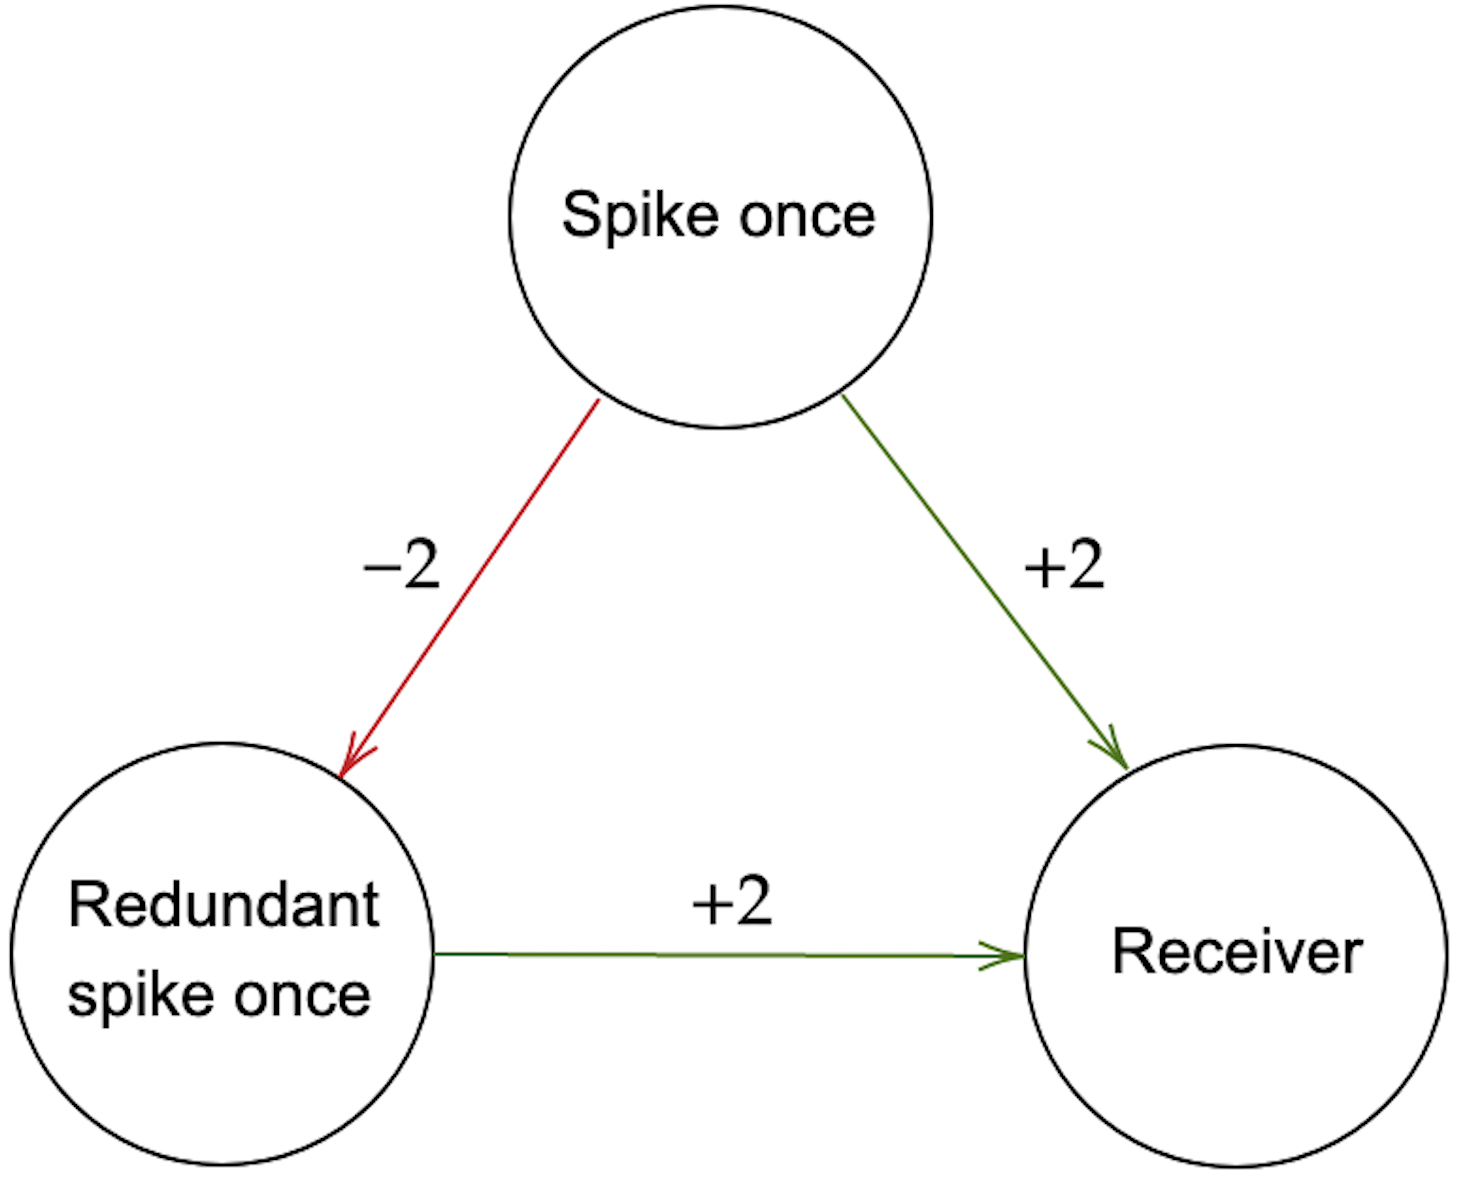
\includegraphics[width=.5\linewidth]{latex/Images/brain_adaptation_alternative.png}
    \caption{Alternative neural pathway for a redundancy of the spike\_once neuron. If the spike\_once neuron dies due to simulated radiation-induced SEEs ($vth=inf$), the redundancy neuron inhibition is eliminated. Without inhibition, the redundant spike\_once neuron copies the spike\_once behaviour with a delay of 1 timestep.}
    \label{fig:eg_brain_adaptation}
\end{figure}

\noindent The alternative neural pathway renders a single neuron $original_i$ with $a$ input synapses, and $b$ output synapses, redundant at the cost of $2a+2b$ synapses and 2 neurons. This cost can be reduced by implementing a controller that scans the network and manually redirects neural pathways to a smaller buffer network. However, that shifts the radiation robustness problem as that controller may also endure SEEs. % This does allow local shielding to be used, and may use components that are physically more robust than the SNN networks.
One can also add triple/$n$-factor redundancy by including more redundant spike\_once neurons that are inhibited by the original spike\_once neuron and each other. This induces an additional delay of t=1 time step per redundant neuron.

%\item \textcolor{red}{An Neumann monitoring module that scans the entire SNN network probing its behaviour, and re-routing broken neurons and/or synapses to redundant neurons.}
%\item \textcolor{red}{A rate-coding frequency adaptation to reduce the relative impact of radiation induced spike omission in a subnetwork of the complete SNN implementation of the MDS approximation.}

\section{Results}\label{sec:results}
%The domains specified in \cref{subsec:results_energy_consumption} to \cref{subsec:results_radiation_robustness} are evaluated as part of the presentation of the results of this experiment. The first three are used to put the radiation robustness in perspective. All four domains are compared to the reference baseline presented in \cref{sec:methodology}.

\subsection{Energy Consumption}\label{subsec:results_energy_consumption}
Barchart here: x-axis: radiation death percentage, per x-coordinate, 3 bars: 10\%,100\%,200\% redundancy, y-axis: percentage of correctly evaluated graphs.

If if multiple 
%\textit{Depending on the radiation test method, the energy consumption may be monitored hardwarematically, or estimated softwarematically. This may be challenging in the case of reliance on neuromorphic cloud architectures for testing, as some may not provide the ability to measure and/or report energy consumption. An approximation to the energy consumption could be counting the occurrence of neuron spikes. This is because neuromorphic architectures are considered to only consume significant amounts of energy when they spike.}

\subsection{Neuronal \& Synaptic Overcapacity}\label{subsec:results_neuronal_synaptic_overcapacity}
By taking this factor into account, a context can be provided for the added value of using brain-inspired radiation robustness implementations in neuromorphic hardware.

\subsection{Traditional Hardware Element Performance}\label{subsec:results_traditional_hardware_element_performance}
\textit{Typical neuromorphic hardware still contains some traditional/Von Neumann architecture components, such as a memory bus and processor. These are typically used to communicate with the outside world, and to orchestrate/set up/initialise the neural network \cite{todo}. Given this position high in the functional hierarchy, they may form a critical bottleneck in terms of radiation robustness. To overcome this issue, a recommendation could be included to increase the shielding and/or redundancy of these Von Neumann components, whilst saving mass and redundancy in the spiking neural networks using brain-inspired implementations \cite{johan_kwisthout_personal_corrospondence_feb_15}.}

\subsection{Radiation Robustness}\label{subsec:results_radiation_robustness}
\textit{This section will be used to present the radiation robustness of the tested neuromorphic architectures with- and without brain-inspired implementation.}
\section{Discussion}\label{sec:discussion}
The reliability of the results can be improved by increasing running the algorithm on more and larger graphs. Running on the Loihi 2 using the Lava 0.4.0 Framework may facilitate this. Even though no public SEE propagation mechanisms are known for the Loihi 2 at the time of writing, the representativeness of the simulation can be increased by taking transient effects, synaptic changes, neuron property changes and Von Neumann component malfunctions into account. The current form of redundancy that is implemented is still dependent on particular neuron properties, and no automated method for arbitrary LIF neuron redundancy is presented. A more intelligent adaptation mechanism may allow for a more active neural pathway redirection to realise equivalent robustness levels at a lower neuronal and synaptic overhead. 
%The discussion is used to put the/any radiation robustness differences between using a brain-inspired implementation and regular redundancy in neuromorphic architectures, into perspective. This perspective is generated by discussing the architecture comparison in terms of the characteristics described in \cref{subsec:discussion_performance_trade_off} to \cref{subsec:discussion_space_application_representation_accuracy}.

%\subsection{Performance Trade-Off}\label{subsec:discussion_performance_trade_off}
%\textit{Increasing the radiation resistance of a default neuromorphic implementation requires some effort. In this study, this effort is realised in the form of a brain-inspired implementation. Such an implementation comes at the cost of resources. In this case those resources are neurons, synapses and energy consumption. Since the comparison is made in terms of radiation robustness, it is important to determine whether it is not merely the consumption of extra resources that led to performance differences. In particular, for space applications, it is important to determine whether the resources that are consumed, for example the energy consumption, are worth the benefits. Each space mission will have its own trade-off in these terms, however, this subsection can shed some light on the trade-off costs. In essence a quantitative insight can be given in terms of performance enhancement and energy cost increases. Similarly, a quantitative insight can be provided in terms of performance enhancement, and the increase in required neurons/synapses and/or hardware mass (if the increase in neurons/synapses require a larger chip).}

%\subsection{Simulation vs Radiation Testing}
%\textit{If the radiation testing is performed softwarematically in this article submission, this section can be used to convey how portable these results are expected to be to practical radiation tests.}

%\subsection{Radiation Robustness of Traditional Hardware Elements}
%\textit{The potential bottleneck of traditional Von Neumann hardware elements in neuromorphic hardware, as introduced in \cref{subsec:results_traditional_hardware_element_performance} should be discussed in this section.}

%\subsection{Space Application Representation Accuracy}\label{subsec:discussion_space_application_representation_accuracy}
%\textit{Some context can be provided in this section to indicate how/up to what extent the radiation testing that is performed for this article submission applies to real space applications.}
% Explain actual space applications may be more AI and less optimisation.
\section{Conclusion}\label{sec:conclusion}
% Talk about results.
%The results presented in \cref{sec:results}, along with their critical context described in \cref{sec:discussion} are to be synthesised in this section to provide a clear insight into the benefits and drawbacks of leveraging implementations inspired by principles of brain adaptation in neuromorphic hardware to increase the radiation robustness of these architectures in space applications.
% Talk about discussion
% Mention whether or not it helped.
Brain-inspired adaptation mechanisms may be used in SNN implementations of graph optimisation problems to increase the radiation robustness of neuromorphic space hardware if SEE propagations can lead to neuron death. Creating more intelligent adaptation mechanisms than separate redundant neuronal pathways for each neuron may improve the radiation results at a lower neuronal overhead. 

% Don't mention that symmetries in distributed algorithms may also be leveraged in lowering the cost of these brain adaptations. Not a conclusion, not mentioned before, not related to this work.

% TODO: write something about overhead and spike energy.
\section{Future Work}\label{sec:recommendations}
%\textit{Recommendations may be generated based on the listed issues in \cref{sec:discussion}. It is foreseeable that dedicated shielding and or redundancy of critical elements of traditional Von Neumann elements in neuromorphic architectures may be advisable, whilst relying on the brain-inspired implementations in SNNs. Another recommendation that may flow out of this research may concern the integration of brain adaptation principles into the design of SNN implementations that yield space application functionalities. Furthermore, a recommendation may be generated regarding a proposed shift in the moment of training, from pre-trained on the ground, to (re-)training after radiation exposure.}

The overarching research project aims to perform physical radiation tests to gain more insight in the practical usefulness of brain-inspired adaptation mechanisms to hedge against radiation damage in neuromorphic space hardware. Since these tests are costly, a more thorough analysis on a broader scope of adaptation mechanisms is proposed. In particular, the population coding and rate coding options will be explored, and the focus is shifted to more AI oriented applications. \cref{subsec:algorithm_selection} to  \cref{subsec:physical_testing}. 





%\begin{acks}
  I would like to acknowledge Elia Montanari and the SpaceBrains foundation for enabling me to pursue this work. Nathal Dorval from ESA for providing me with feedback on my progress during this work. Dr. J.H.P. Kwisthout for consistently and kindly providing me with feedback and guidance. Dr. D.M. Stam for enabling me to pursue this research from the earliest conception of the idea, and Dr. A. Menicucci for providing me with technical and strategic advice throughout this project.
\end{acks}
\fi



%%
%% The acknowledgments section is defined using the "acks" environment
%% (and NOT an unnumbered section). This ensures the proper
%% identification of the section in the article metadata, and the
%% consistent spelling of the heading.
\ifx\homepath\overleafhome
% Overleaf compilation.

% Include chapters.
%\begin{abstract}
  %Energy efficient applications of artificial intelligence (AI) may be able to increase space robot autonomy. 
  This research sets out to test whether principles of brain adaptation can be leveraged to increase the radiation resistance of neuromorphic space hardware. Neuromorphic architectures provide energy efficient platforms for AI applications in space. Structural similarities between neuromorphic architectures and the brain may allow them to benefit from brain-inspired design on the topic of damage recovery. Space environments can provide challenging conditions with significant radiation exposure, that may damage neuromorphic space hardware. A brain-inspired approach is explored in mitigating such damage.
  
  This approach is investigated using simulated radiation robustness tests with- and without brain adaptation implementation. The differences in radiation robustness are then analysed and discussed in the context of space applications of neuromorphic hardware. The SNN implementation by Diehl et al. of the minimum dominating set approximation algorithm by Alipour et al. is enhanced with brain adaptation mechanisms for these tests \cite{alipour2020distributed}\cite{diehl}. The tests are performed using Intel's Lava framework V0.3.0.
\end{abstract}
\begin{acks}
  I would like to acknowledge Elia Montanari and the SpaceBrains foundation for enabling me to pursue this work. Nathal Dorval from ESA for providing me with feedback on my progress during this work. Dr. J.H.P. Kwisthout for consistently and kindly providing me with feedback and guidance. Dr. D.M. Stam for enabling me to pursue this research from the earliest conception of the idea, and Dr. A. Menicucci for providing me with technical and strategic advice throughout this project.
\end{acks}
\else
% Local compilation

% Include chapters.
%\begin{abstract}
  %Energy efficient applications of artificial intelligence (AI) may be able to increase space robot autonomy. 
  This research sets out to test whether principles of brain adaptation can be leveraged to increase the radiation resistance of neuromorphic space hardware. Neuromorphic architectures provide energy efficient platforms for AI applications in space. Structural similarities between neuromorphic architectures and the brain may allow them to benefit from brain-inspired design on the topic of damage recovery. Space environments can provide challenging conditions with significant radiation exposure, that may damage neuromorphic space hardware. A brain-inspired approach is explored in mitigating such damage.
  
  This approach is investigated using simulated radiation robustness tests with- and without brain adaptation implementation. The differences in radiation robustness are then analysed and discussed in the context of space applications of neuromorphic hardware. The SNN implementation by Diehl et al. of the minimum dominating set approximation algorithm by Alipour et al. is enhanced with brain adaptation mechanisms for these tests \cite{alipour2020distributed}\cite{diehl}. The tests are performed using Intel's Lava framework V0.3.0.
\end{abstract}
\begin{acks}
  I would like to acknowledge Elia Montanari and the SpaceBrains foundation for enabling me to pursue this work. Nathal Dorval from ESA for providing me with feedback on my progress during this work. Dr. J.H.P. Kwisthout for consistently and kindly providing me with feedback and guidance. Dr. D.M. Stam for enabling me to pursue this research from the earliest conception of the idea, and Dr. A. Menicucci for providing me with technical and strategic advice throughout this project.
\end{acks}
\fi


%%
%% The next two lines define the bibliography style to be used, and
%% the bibliography file.
\bibliographystyle{ACM-Reference-Format}
%\bibliography{sample-base}
\bibliography{zotero}

%%
%% If your work has an appendix, this is the place to put it.
\appendix

%\section{Research Methods}

%\subsection{Part One}

%Lorem ipsum dolor sit amet, consectetur adipiscing elit. Morbi
%malesuada, quam in pulvinar varius, metus nunc fermentum urna, id
%sollicitudin purus odio sit amet enim. Aliquam ullamcorper eu ipsum
%vel mollis. Curabitur quis dictum nisl. Phasellus vel semper risus, et
%lacinia dolor. Integer ultricies commodo sem nec semper.
%
%\subsection{Part Two}
%
%Etiam commodo feugiat nisl pulvinar pellentesque. Etiam auctor sodales
%ligula, non varius nibh pulvinar semper. Suspendisse nec lectus non
%ipsum convallis congue hendrerit vitae sapien. Donec at laoreet
%eros. Vivamus non purus placerat, scelerisque diam eu, cursus
%ante. Etiam aliquam tortor auctor efficitur mattis.
%
%\section{Online Resources}
%
%Nam id fermentum dui. Suspendisse sagittis tortor a nulla mollis, in
%pulvinar ex pretium. Sed interdum orci quis metus euismod, et sagittis
%enim maximus. Vestibulum gravida massa ut felis suscipit
%congue. Quisque mattis elit a risus ultrices commodo venenatis eget
%dui. Etiam sagittis eleifend elementum.
%
%Nam interdum magna at lectus dignissim, ac dignissim lorem
%rhoncus. Maecenas eu arcu ac neque placerat aliquam. Nunc pulvinar
%massa et mattis lacinia.

\end{document}
\endinput
%%
%% End of file `sample-sigconf.tex'.